%%%%%%%%%%%%%%%%%%%%%%%%%%%%%%%%%%%%%%%%%%%%%%%%%%%%%%%%%%%%%%%%%
%
% Project     : Turnverein App
% Title       : 
% File        : projektplanung.tex Rev. 00
% Date        : 07.07.14
% Author      : Raffael Santschi
%
%%%%%%%%%%%%%%%%%%%%%%%%%%%%%%%%%%%%%%%%%%%%%%%%%%%%%%%%%%%%%%%%%

\chapter{Projektplanung}\label{chap.projektplanung}
Dieses Kapitel handelt von der Projektplanung und den verschiedenen Arbeitspaketen in diesem Projekt.

\section{Meilensteine}\label{meilensteine}
Folgende Meilensteine wurden für dieses Projekt festgelegt:

\begin{table}[ht]
\centering
  \begin{tabular}{ l | r }
	\hline
	\rowcolor{gray}
	Projektstart:					&	01.04.2014	\\ \hline
	Anforderungsdokument Entwurf		&	07.05.2014	\\ \hline
	Anforderungsdokument fertig		&	12.07.2014	\\ \hline
	Refactoring abgeschlossen		&	04.08.2014	\\ \hline
	App und Backend implementiert		& 	30.08.2014	\\ \hline
	Test-Phase abgeschlossen			&	02.09.2014	\\ \hline
	App zur Freigabe eingesendet		&	02.09.2014	\\ \hline
	Dokumentation fertig			&	20.09.2014	\\ \hline
	Dokumentation korrigiert			&	27.09.2014	\\ \hline
  \end{tabular}
   \caption{Meilensteine}\label{table:milestones}
\end{table}

\section{Arbeitspakete}\label{arbeitspakete}
Das Projekt beinhaltet sechs Arbeitspakete:
\begin{itemize}
\item Planung
\item Requirement Engineering
\item Refactoring Backend
\item Entwicklung Mobile App
\item Testing
\item Dokumentation
\end{itemize}

\subsection{Planung}\label{planung}
In der Planungsphase wird geschaut, was in dem Projekt erreicht werden muss und wie diese Tätigkeiten auf die vorhandene Zeit aufgeteilt wird. Es wird auch das erste Mal mit den Stakeholdern geredet und erste Abmachungen getroffen.

\subsection{Requirement Engineering}\label{rqe}
Bei der Erstellung eines neuen Systems ist es immer wichtig, dass man alle Anforderungen kennt. Um die Anforderungen zu erfassen werden die Mitglieder und der Vorstand befragt, was sie sich von der App wünschen. Die Mitglieder sind nur zum Teil Techniker, somit werden auch Anforderungen resultieren, welche sehr schwierig umzusetzen sind und andere Anforderungen werden nicht aufgelistet, sondern einfach vorausgesetzt, sogenannte Basisfaktoren. Der Anforderungskatalog wird mit den Mitgliedern, welche sich eingebracht haben, angeschaut und am Schluss findet ein Review statt. (siehe dazu auch \cite{req_eng_book})

\subsection{Refactoring Backend}\label{ref_backend}
Als erste Entwicklungstätigkeit muss das Backend umgebaut werden, damit die Implementation für die App leichter fällt. Dazu wird der Ist-Stand aufgenommen und geschaut, welche Klassen umstrukturiert werden müssen, damit die Implementation danach leichter fällt. Danach wird entschieden, welches Pattern man beim Umbau der Klassen verfolgen möchte. Das Umbauen selbst ist mit viel Arbeit und Testen verbunden.

\subsection{Entwicklung Mobile App}\label{eng_app}
In diesem Arbeitspaket werden die Anforderungen umgesetzt. Die App wird entworfen und mit Inhalt gefüllt. Die ersten Tests werden durchgeführt und Unstimmigkeiten in den Anforderungen mit den Stakeholdern angeschaut.

\subsection{Tests}\label{tests}
Es gibt zwei Testsphasen, die eine ist dann, wenn das neue Backend online ist und die User, wie gewohnt, arbeiten können sollten. Die andere besteht darin, dass die App für Android zum Download bereit gestellt wird, nachdem die ersten Tests erfolgreich waren.  Das Feedback wird bei beiden Phasen eingearbeitet und möglichst schnell aktualisiert.

\subsection{Dokumentation}\label{dokumentation}
Die Dokumentation wird das ganze Projekt hindurch aktuell gehalten. Für das Erfassen dieses Dokuments wird \LaTeX\ und das \LaTeX-Template der ZHAW verwendet.


\newpage
\section{Projektstrukturplan}\label{projektstrukturplan}
Anhand der Arbeitspaketen wurde ein Projektstrukturplan (siehe Abbildung \ref{fig:psp}) erstellt, welcher die Arbeitspakete in Teilaufgaben unterteilt. Diese Methode ist aus \cite{proj_mgmt_book} bekannt.
\begin{figure}[h]
\centering
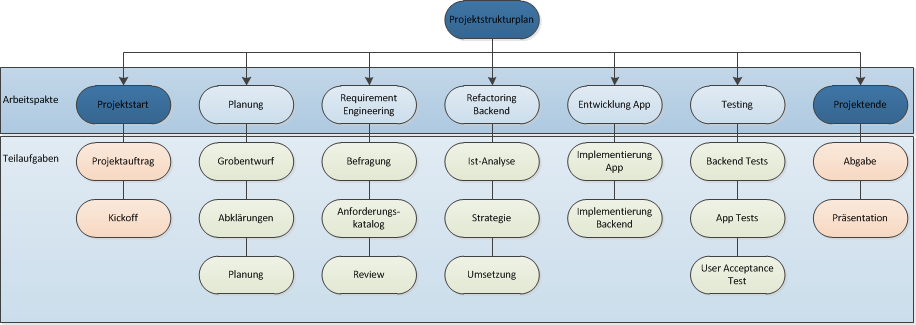
\includegraphics[scale=0.7]{images/visio/PSP.png}
\caption{Projektstrukturplan}
\label{fig:psp}
\end{figure}



\section{Zeitplan}\label{zeitplan}
Der Zeitplan gibt eine grobe Übersicht, wann an dem Projekt gearbeitet wird und wann die verschiedenen Tätigkeiten fertig werden. Die Angaben sind nur Richtwerte, da neben diesem Projekt noch einer Arbeit nachgegangen wird, verschiedenen Tätigkeiten im Verein ausgeführt werden und zusätzliche andere Arbeiten und Prüfungen Zeit benötigen.

\subsection{Geplante Abwesenheiten}
\begin{table}[ht]
\centering
  \begin{tabular}{ l | r }
	\hline
	\rowcolor{gray}
	Abwesenheit							&	Start - Ende	\\ \hline
	Seminararbeit Abgaben					&	01.06.2014 - 22.06.2014	\\ \hline
	Modulprüfungen und Vorträge Seminararbeit		&	23.06.2014 - 02.07.2014	\\ \hline
	Ferien								&	12.07.2014 - 03.08.2014	\\ \hline
  \end{tabular}
   \caption{Geplante Abwesenheiten}\label{table:holidays}
\end{table}

\begin{landscape}
\thispagestyle{empty}
\subsection{Projektplan}\label{projektplan}
Der Zeitplan basierend auf dem Projektstrukturplan (siehe \ref{projektstrukturplan})  und den geplanten Abwesenheiten sieht wie folgt aus:
\begin{figure}[h]
\centering
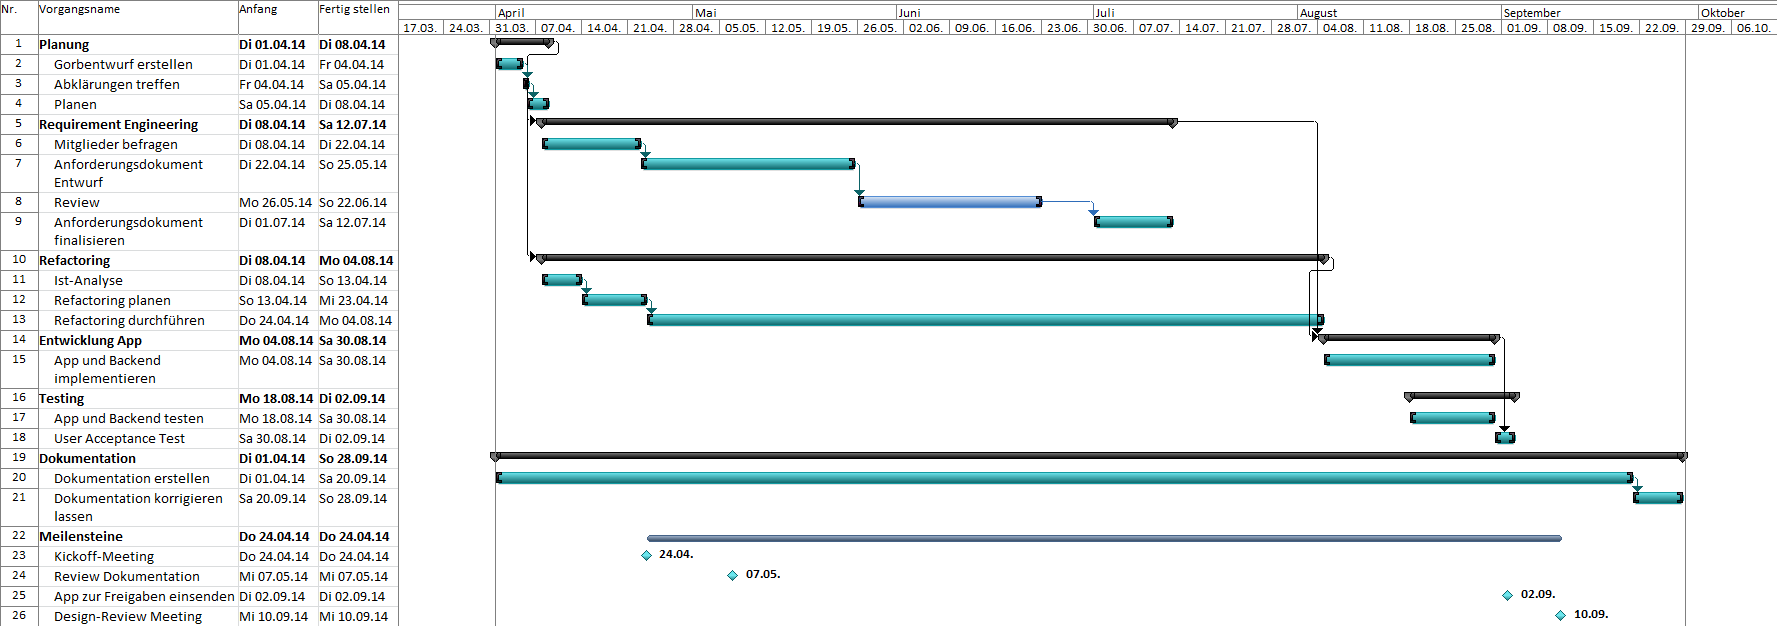
\includegraphics[scale=0.5]{images/project/projectplan.png}
\caption{Projektplan}
\label{fig:psp}
\end{figure}

\end{landscape}

\subsection{Zeitschätzung auf Arbeitspaketebene}
\begin{table}[ht]
\centering
  \begin{tabular}{ l | c | c }
	\hline
	\rowcolor{gray}
	Arbeitspaket							&	Schätzung (h)	& Tatsächlich (h)	\\ \hline
	Planung							&	10			& 8	\\ \hline
	Requirement Engineering					&	12			& 15	\\ \hline
	Refactoring Backend					&	20			& 40	\\ \hline
	Entwicklung Mobile App					&	45			& 50	\\ \hline
	Tests								&	8			& 10	\\ \hline
	Dokumentation						&	60			& 70	\\ \hline \hline
	Total								&	155			& 193	\\ \hline
  \end{tabular}
   \caption{Zeitschätzung auf Arbeitspaketebene}\label{table:time_estimation}
\end{table}

\section{Risikoanalyse}\label{risikoanalyse}
Jedes Projekt birgt Risiken. Werden diese nicht am Anfang analysiert und über die gesamte Projektlaufzeit überwacht, kann es zu grossen Schwierigkeiten kommen. Die angewandten Methoden sind aus \cite{proj_mgmt_book} und aus dem Management Fach Projekt und Prozessmanagement bekannt.

\subsection{Risikoermittlung}\label{risikoermittlung}
Die Risikoermittlung ist dafür da, dass man mögliche Risiken aufdeckt und die möglichen Folgen daraus festhält.

\begin{table}[ht]
\centering
  \begin{tabular}{  p{5cm} | p{9cm} }
	\hline
	\rowcolor{gray}
	Risiko							&	Mögliche Folgen	\\ \hline
	Implementationsschwierigkeiten (Nur wenig Erfahrung in der App Entwicklung)
								&	\begin{itemize}
										\item Zeitplan nicht einhaltbar
										\item Einige Anforderungen müssen zurück gestellt werden
										\item Projektarbeit kann nicht durchgeführt werden
									\end{itemize}	\\ \hline
	Ressourcen nicht verfügbar
								&	\begin{itemize}
										\item Zeitplan nicht einhaltbar
										\item Einige Anforderungen müssen zurück gestellt werden
										\item Projektarbeit kann nicht durchgeführt werden
									\end{itemize}	\\ \hline
	Mangelhaftes Endprodukt		
								&	\begin{itemize}
										\item Produkt muss überarbeitet werden, da keine Abnahme durch die Stakeholder erfolgt
									\end{itemize}	\\ \hline	
	Anforderungen nicht vollständig	
								&	\begin{itemize}
										\item Wichtige Funktionen stehen den Benutzern nicht zur Verfügung
									\end{itemize}	\\ \hline			
  \end{tabular}
   \caption{Risikoermittlung}
\end{table}

\subsection{Risikobewertung}
Das Schadensausmass und die Eintrittswahrscheinlichkeit der Risiken sind nach folgendem Schema bewertet worden:

\begin{table}[ht]
\centering
  \begin{tabular}{ l | p{5cm} | p{5cm} }
	\hline
	\rowcolor{gray}
	Wert							&	Eintrittswahrscheinlichkeit		&	Schadensausmass	\\ \hline			
	1							&	sehr unwahrscheinlich		&	vernachlässigbar	\\ \hline
	2							&	unwahrscheinlich			&	spürbar		\\ \hline
	3							&	wenig wahrscheinlich		&	verkraftbar		\\ \hline
	4							&	ziemlich wahrscheinlich		&	gefährlich		\\ \hline
	5							&	sehr wahrscheinlich			&	katastrophal		\\ \hline
  \end{tabular}
   \caption{Risikobewertungsschema}
\end{table}

\FloatBarrier
Die Risiken aus der Risikobewertung (siehe \ref{risikoermittlung}) wurden anhand dieses Schemas bewertet.

\begin{equation*}
Risikofaktor = Eintrittswahrscheinlichkeit * Schadensausmass
\end{equation*}

\begin{table}[ht]
\centering
  \begin{tabular}{ l | p{4cm} | p{3cm} | c }
	\hline
	\rowcolor{gray}
	Risiko							&	Eintrittswahrscheinlichkeit		&	Schadensausmass 	&	Risikofaktor\\ \hline			
	Implementationsschwierigkeiten			&	1					&	4			&	4		\\ \hline
	Ressourcen nicht verfügbar			&	2					&	5			&	\textbf{10}	\\ \hline
	Mangelhaftes Endprodukt				&	2					&	4			&	\textbf{8}	\\ \hline
	Anforderungen nicht vollständig			&	3					&	3			&	\textbf{9}	\\ \hline
  \end{tabular}
   \caption{Risikobewertung}
\end{table}

\subsection{Risikomatrix}
Anhand der Risikobeurteilung konnten die Risiken in eine Risikomatrix eingesetzt werden. Diese Matrix bietet einen guten Überblick über die Risiken und zeigt schnell, welche Risiken beachtet werden müssen.
\begin{figure}[h]
\centering
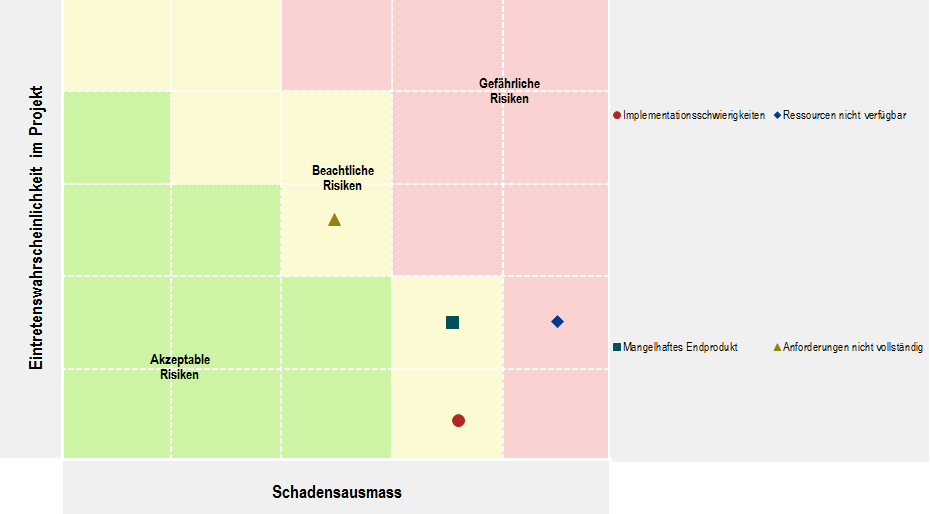
\includegraphics[scale=0.5]{images/excel/risikomatrix.png}
\caption{Risikomatrix}
\label{fig:risikomatrix}
\end{figure}

\subsection{Massnahmen}
Es wurden Massnahmen für die gefundenen Risiken gesucht und festgehalten. Die Massnahmen sind wiederum in vorbeugende Massnahmen und Eventual-Massnahmen unterteilt.

\begin{table}[ht]
\centering
  \begin{tabular}{  l | p{4cm} | p{4cm} }
	\hline
	\rowcolor{darkgray}
	Risiko							&	\multicolumn{2}{|c|}{Massnahmen} \\ \hline
	\rowcolor{gray}
								&	Vorbeugende Massnahmen & Eventual-Massnahmen	\\ \hline
	Implementationsschwierigkeiten
								&	\begin{itemize}
										\item Im Zeitplan genügend Reserven einrechnen
										\item Kontaktpersonen zum Thema suchen
									\end{itemize}
								&	\begin{itemize}
										\item Betreuer / Schulleitung informieren
										\item Verschiebungsgesuch stellen
									\end{itemize}						\\ \hline
	Ressourcen nicht verfügbar
								&	\begin{itemize}
										\item Fixe Zeiten einplanen
										\item Tätigkeiten priorisieren
									\end{itemize}
								&	\begin{itemize}
										\item Verschiebungsgesuch mit guter Begründung stellen
									\end{itemize}	\\ \hline
	Mangelhaftes Endprodukt		
								&	\begin{itemize}
										\item Anforderungskatalog sauber erstellen
										\item Testphase möglichst früh beginnen, damit noch genügen Zeit für die Einarbeitung des Feedbacks ist
									\end{itemize}
								&	\begin{itemize}
										\item Lösung mit dem Kunden suchen
										\item Projekt verlängern
									\end{itemize}	\\ \hline	
	Anforderungen nicht vollständig	
								&	\begin{itemize}
										\item Review des Anforderungskataloges
										\item Testphase möglichst früh beginnen, damit noch genügen Zeit für die Einarbeitung des Feedbacks ist
									\end{itemize}
								&	\begin{itemize}
										\item Anforderungen werden aufgenommen und in einen nächsten Release geplant											
									\end{itemize}	\\ \hline			
  \end{tabular}
   \caption{Risikoanalyse - Massnahmen}
\end{table}


